\section{Problem 1}
\textit{Look at the code and try to sketch (graphically) the scattering layout it is implementing.}\\

The scattering layout being implemented is two sets of scatterers, each set form a ring around an array of 4 antennas (4 antennas transmitting and 4 receiving in total). The code allows the user to control the number of scatterers around the arrays of antennas; the distance between the center of the rings; the distance traveled by the arrays of antennas. An example is shown in figure \figref{fig:2D_setup1}.

\begin{figure}[!h]
  \centering
  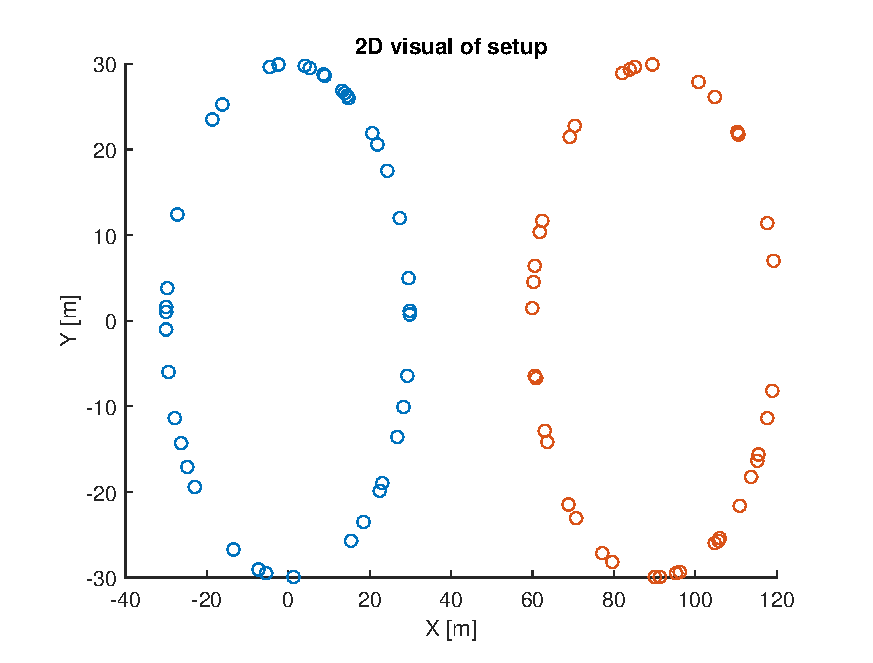
\includegraphics[width=10cm]{2D_setup1.eps}
  \caption{Example of the layout of the simulation.}
  \label{fig:2D_setup1}
\end{figure}

\subsection{a)}
\textit{Find link correlations (complex, envelope or power. What do you choose/why?)}\\

The correlation of envelope and power due to it is easy to treat and in most cases it is sufficient.
In \figref{fig:Envelope} the correlation between h11 and h32 has been calculated, and is shown in the plot.
\begin{figure}[!h]
  \centering
  \includegraphics[width=10cm]{envelope.eps}
  \caption{Envelope of four links, and the correlation between h11 and h32}
  \label{fig:Envelope}
\end{figure}

\subsection{b)}
\textit{Look at eigen distribution, what is seen?}\\

The eigen distribution is sown in the following for the two "extremes". The first, where there is a very good mixing of the paths and we will see all four modes. And the second, where the keyhole effect can bee seen. These two have been produced by different "engines" in the code to produce the specific outcomes. The two engine $h_1$ and $h_2$ can be seen in the following:

\code{language=Matlab,caption = The two eninges,label=cl:imp_resp_code,linerange={65-75},firstnumber=65}{code/mm9/Dual_ring.m}

\begin{figure}[!h]
  \centering
  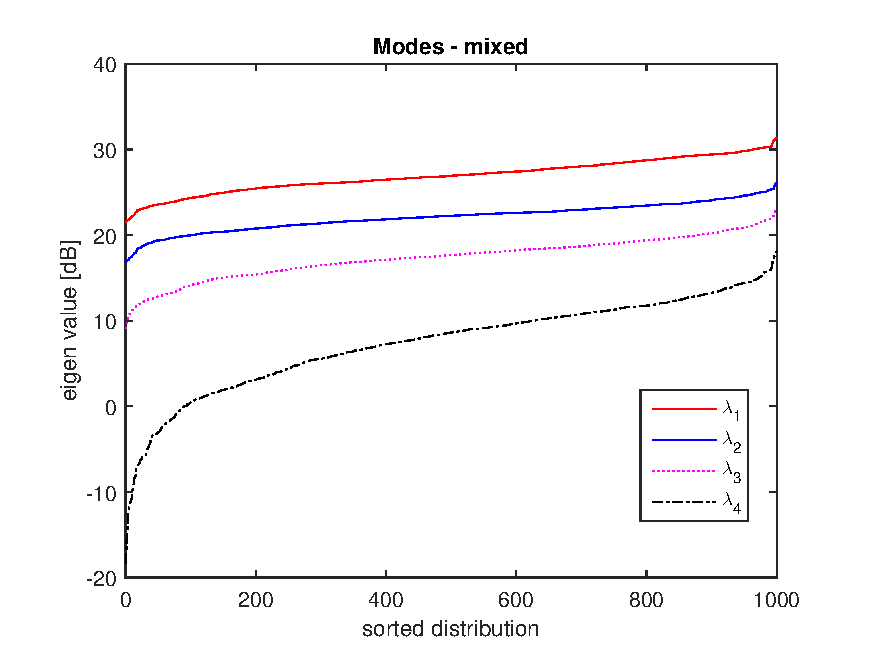
\includegraphics[width=10cm]{modes_mixed.eps}
  \caption{The eigenmodes in mixed environment, all four modes possible}
  \label{fig:modes_mixed}
\end{figure}

\begin{figure}[!h]
  \centering
  \includegraphics[width=10cm]{modes_keyhole.eps}
  \caption{The eigenmodes in "keyhole" effect, only one mode possible}
  \label{fig:modes_mixed}
\end{figure}

\subsection{c)}
\textit{What is envelope distribution of link signals (in dB , why?)? (look at 10\% level vs mean, why?)}\\

The first "engine" $h_1$, in the code will produce the single Rayleigh, while the second "engine", $h_2$, is used for the dual Rayleigh.

\begin{figure}[!h]
  \centering
  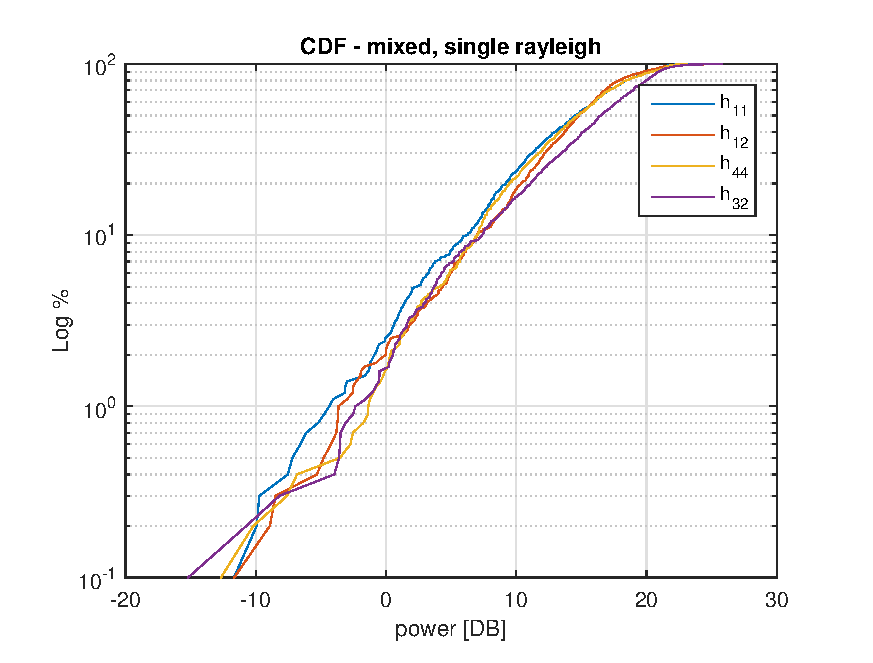
\includegraphics[width=10cm]{cdf_rayleigh.eps}
  \caption{Single-Rayleigh from the $h_1$ engine in the code}
  \label{fig:modes_mixed}
\end{figure}

\begin{figure}[!h]
  \centering
  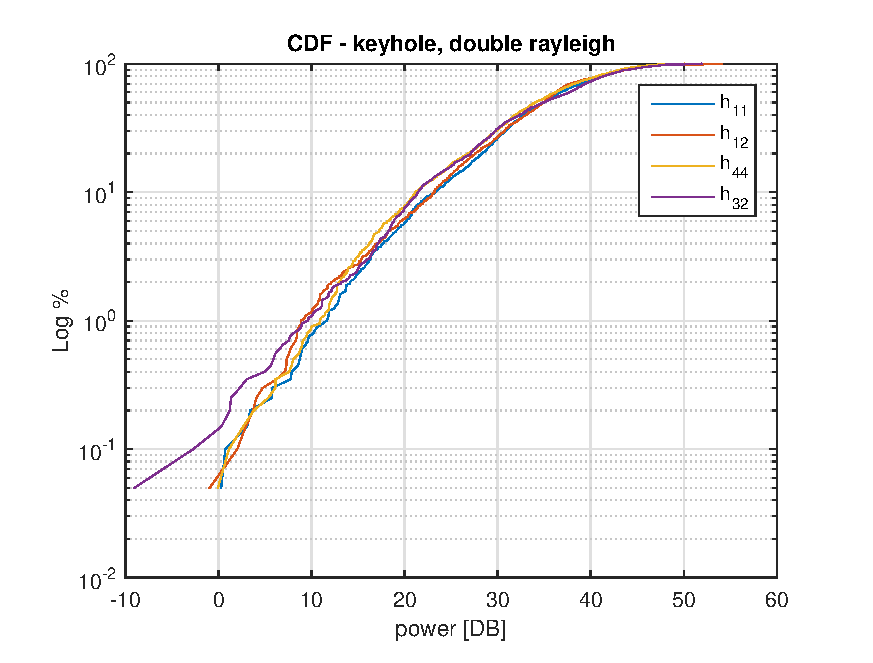
\includegraphics[width=10cm]{cdf_double_rayleigh.eps}
  \caption{Double-Rayleigh from the $h_2$ engine in the code}
  \label{fig:modes_mixed}
\end{figure}

\subsection{d)}
\textit{Doppler spectrum of a link signal looks like??}\\

The Doppler spectrum of a link signal has the classical bathtub shape when only one of the antennas array is moving; this can be seen in \figref{fig:singledopp}. When both antennas arrays are moving, the shape of the observed Doppler spectrum is the ``tent shape'' as the studied Double-Doppler effect. This can be seen in \figref{fig:dualdopp}

\begin{figure}[!h]
  \centering
  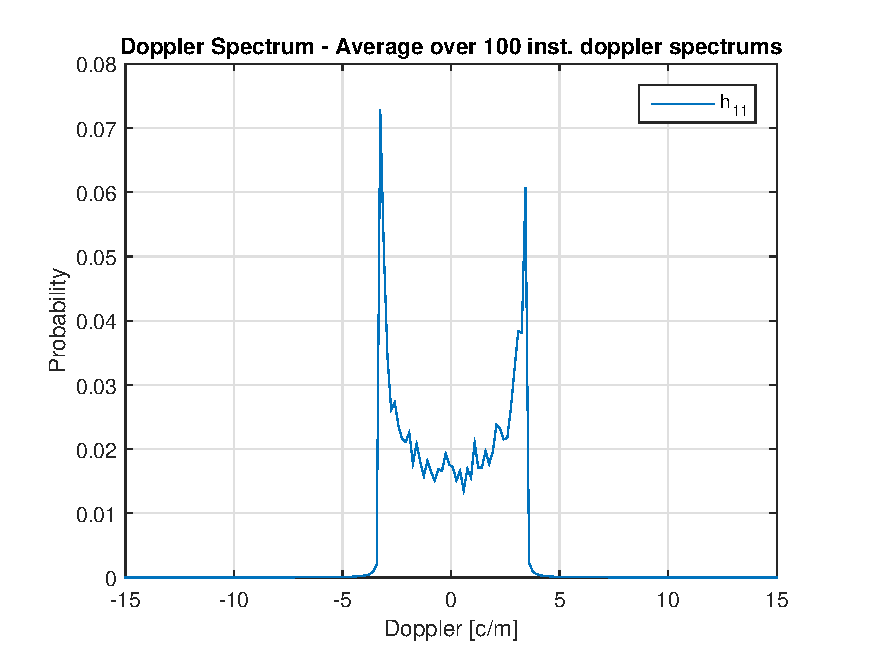
\includegraphics[width=10cm]{singledopp.eps}
  \caption{Doppler spectrum of a link when only one array is moving. "Bathtub shape" can be appreciated.}
  \label{fig:singledopp}
\end{figure}

\begin{figure}[!h]
  \centering
  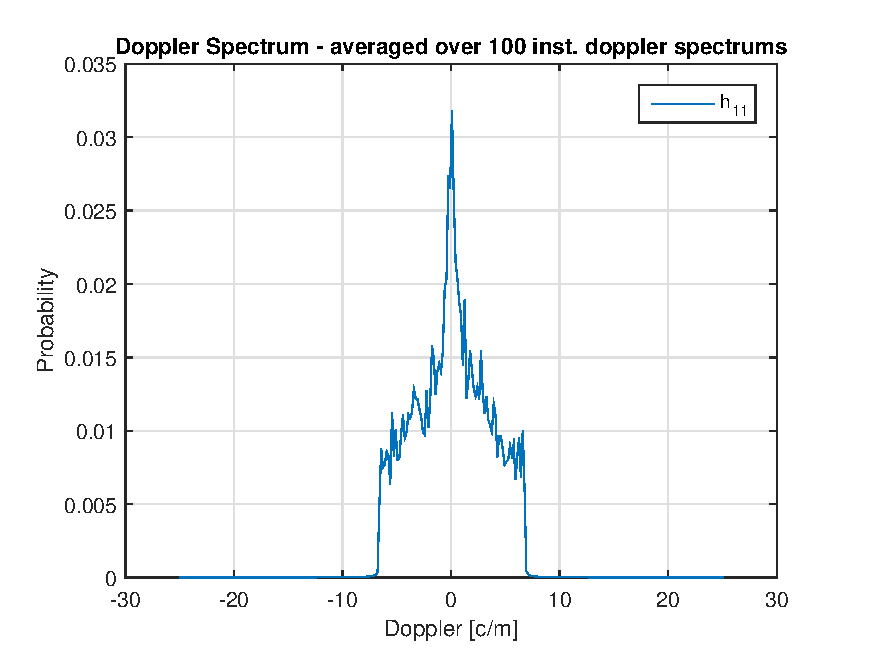
\includegraphics[width=10cm]{dualdopp.eps}
  \caption{Doppler spectrum of a link when both array is moving. "Tent shape" can be appreciated.}
  \label{fig:dualdopp}
\end{figure}

\subsection{e)}
\textit{Identify channel type (based on sketch and/or eigen distribution etc)}\\

As already have been seen through these exercises, we have identified both "mixed" and "tubes" channel types. The two extremes have been demonstrated in the Doppler spectrums and the plot of the eigenmodes.